% arara: xelatex: { shell : yes }
% arara: biber
% arara: xelatex: { shell : yes }
% arara: xelatex: { shell : yes }

% options:
% thesis=B bachelor's thesis
% thesis=M master's thesis
% czech thesis in Czech language
% slovak thesis in Slovak language
% english thesis in English language
% hidelinks remove colour boxes around hyperlinks

\documentclass[thesis=B,czech]{FITthesis}[2019/12/23]

% \usepackage{amsmath} %advanced maths
% \usepackage{amssymb} %additional math symbols

\usepackage{dirtree} %directory tree visualisation

% % list of acronyms
% \usepackage[acronym,nonumberlist,toc,numberedsection=autolabel]{glossaries}
% \iflanguage{czech}{\renewcommand*{\acronymname}{Seznam pou{\v z}it{\' y}ch zkratek}}{}
% \makeglossaries

\newcommand{\tg}{\mathop{\mathrm{tg}}} %cesky tangens
\newcommand{\cotg}{\mathop{\mathrm{cotg}}} %cesky cotangens

\usepackage[style=iso-numeric,backend=biber]{biblatex}
\addbibresource{mybibliographyfile.bib}
\addbibresource{ref.bib}

% % % % % % % % % % % % % % % % % % % % % % % % % % % % % % 
% ODTUD DAL VSE ZMENTE
% % % % % % % % % % % % % % % % % % % % % % % % % % % % % % 

\department{Katedra softwarového inženýrství}
\title{Automatický provisioning herních serverů pomocí cloudové image}
\authorGN{Matyáš} %(křestní) jméno (jména) autora
\authorFN{Ješina} %příjmení autora
\authorWithDegrees{Matyáš Ješina} %jméno autora včetně současných akademických titulů
\author{Matyáš Ješina} %jméno autora bez akademických titulů
\supervisor{Ing. Tomáš Vondra, Ph.D.}
\acknowledgements{Doplňte, máte-li komu a za co děkovat. V~opačném případě úplně odstraňte tento příkaz.}
\abstractCS{Tato práce se zabývá problematikou automatického nasazování herních serverů a jejich provozu v cloudovém prostředí.
Zkoumá možnosti nasazování aplikací v cloudu za účelem nalezení nejefektivnějšího způsobu
a popisuje vytvoření obrazu systému, který je pro dané využití vhodný. Tento systém je schopný podporovat množství herních serverů
bez nutnosti jeho časté změny a je snadno rozšiřitelný i pro další hry v budoucnosti.

Výsledkem je obraz systému určeného pro provoz herních serverů, který je bezpečný, obsahuje jen nezbytně nutné součásti a dá se jednoduše nasadit v cloudovém prostředí.
Celý proces jeho sestavení je plně automatizovaný.}
\abstractEN{This thesis addresses the possibilities of automatic deployment and provisioning of game
servers in cloud environment. It explores existing possibilities of deploying applications in cloud to find the optimal solution
and describe the creation of a system image appropriate for this use case. This system is capable of running various game servers without frequent
changes to its internal structure and is easily modifiable to include more games, if desired.

The result si a system image designated to run game servers, which is secure,
contains only the most necessary components, and can easily be deployed to cloud environment. The entire
process is fully automated.}
\placeForDeclarationOfAuthenticity{V~Praze}
\declarationOfAuthenticityOption{4} %volba Prohlášení (číslo 1-6)
\keywordsCS{herní server, počítačová hra, cloud, automatizace, nasazování systému}
\keywordsEN{game server, video game, cloud, automatization, system deployment}
% \website{http://site.example/thesis} %volitelná URL práce, objeví se v tiráži - úplně odstraňte, nemáte-li URL práce
\usepackage{csquotes} % dává české enquotes
\usepackage{xevlna}

\begin{document}

% \newacronym{CVUT}{{\v C}VUT}{{\v C}esk{\' e} vysok{\' e} u{\v c}en{\' i} technick{\' e} v Praze}
% \newacronym{FIT}{FIT}{Fakulta informa{\v c}n{\' i}ch technologi{\' i}}

\begin{introduction}

Počítačové hry se těší velké popularitě. S rozšířením internetu začaly vznikat také hry
pro více hráčů, které se rychle dostaly do čela žebříčků oblíbenosti a dnes jsou zábavou pro stovky milionů
hráčů po celém světě.

Mnohé z těchto her umožňují uživatelům vytvořit vlastní herní servery, na kterých je možné hrát s přáteli
či jinou komunitou.

Pokud chce uživatel zprovoznit herní server, měl by takový postup být jednoduchý a rychlý.
Existuje zde například možnost provozu serveru na vlastním počítači, zde je však kvalita herního zážitku 
ovlivněna konfigurací systému a internetovým připojením. Také je často potřeba pokročilého nastavení
směrovače, který herní server z domácí sítě zpřístupní do internetu.

Tato práce se zaměřuje na další možnost provozu těchto serverů, a to v cloudovém prostředí. Uživatel se tak nemusí zabývat 
kvalitou internetového připojení či manuálním nastavováním síťových prvků. Herní servery
pro menší počet hráčů jsou často vytvářeny a rušeny, nasazení v cloudu tedy představuje ideální způsob provozu,
kde jsou tyto operace jednoduché a automatizovatelné.

Cílem práce je vytvořit obraz systému, který bude pro toto použití vhodný. Uživatel bude mít možnost vybrat
požadovaný herní server a systém provede všechny operace potřebné k jeho zprovoznění.

Výsledek práce bude prospěšný zejména pro stávající uživatele cloudových služeb, kteří mají alespoň minimální
zkušenosti s nasazováním obrazů systémů. S minimální interakcí budou mít možnost spustit herní server dle svého
výběru bez složité instalace a konfigurace. Pokročilí uživatelé využijí možnosti automatizace celého procesu,
která jim zaručí rychlé spuštění vybraného serveru za pomoci několika příkazů.

Vytvořený obraz tedy musí být snadno dostupný a zdokumentovaný, jednoduchý na nasazení, s minimální náročností 
na systémové prostředky. Bude jej také možné využít v komerčním prostředí.

\end{introduction}

\chapter{Cíl práce}

Hlavním cílem této práce je vytvořit obraz systému, který bude schopný provozovat herní servery v cloudovém prostředí.
Tento systém musí být jednoduchý na zprovoznění i úpravy. Bude tedy ideálním kandidátem pro uživatele se základní znalostí
nasazování serverů v cloudu, který nechce provozovat herní server na vlastní infrastruktuře.
Práce se zaměří na herní servery pro menší množství hráčů (přibližně do 50), které obecně vyžadují méně systémových prostředků a nastavení
a proces jejich vytváření je tak jednoduše automatizovatelný.

V první části práce je tedy nutné analyzovat dostupné možnosti a najít výhody a nevýhody daných řešení. Dále je potřeba vybrat
vhodný operační systém, který splňuje dané požadavky. V dalším kroku budou porovnány různé možnosti provozu herních serverů
na daném systému a jejich automatizace.

V praktické části bude implementována součást pro automatickou instalaci herních serverů a jejich provoz. Jelikož je kladen důraz
na jednoduchost provozu, bude tento program pracovat s minimální interakcí uživatele, případně plně automaticky.
Tato součást také musí být schopna spouštět a zastavovat herní server, bude-li to nutné.

Jelikož se bude po nasazení jednat o veřejně dostupný systém, je zde důležitým prvkem jeho bezpečnost. Budou tedy vyhodnoceny možnosti
jeho zabezpečení, zahrnující například vzdálený přístup.

\chapter[Analýza]{Analýza a návrh}

% V této kapitole provedeme analýzu požadavků a návrh včetně zdůvodnění všech rozhodnutí. \cite{efficient_resources}
% \cite{newcombe_2012}
% \cite{building_cloud_mog_server}

V této části budou prozkoumány vhodné operační systémy a existující řešení pro vytváření herních serverů v cloudu.
Bude proveden návrh možného řešení a probrány možné výhody a nevýhody.

\section{Literární rešerše}

Vzhledem k rostoucí popularitě cloudových služeb \cite{statista_cloud_revenue} existuje množství zdrojů, ze kterých lze čerpat.
Herní servery se oproti ostatním typům běžných cloudových aplikací odlišují svojí vysokou náročností
na systémové prostředky, mimo jiné například požadavkem na nízkou latenci.

Při provozování cloudového serveru pro velké množství hráčů je nutné zajistit správné fungování infrastruktury,
jako je například správné vyvažování zátěže mezi jednotlivé servery či automatický výběr nejvhodnějšího serveru
pro klienta \cite{building_cloud_mog_server}. Tyto problémy zde není nutné řešit -- výsledek práce má sloužit jako jednoduchý a rychlý
způsob nasazení herního serveru, není tedy z principu vhodný pro dlouhodobé obsluhování velkého množství hráčů.

U poskytovatelů cloudových serverů je možné vybrat množství systémových prostředků, které bude mít aplikace k dispozici.
Pokud sledujeme vytížení herních serverů v čase, můžeme spatřit jisté vzory, například nárůst hráčů ve večerních hodinách.
Jedná-li se o velký rozdíl v množství uživatelů, je nutné dynamicky navyšovat systémové prostředky \cite{efficient_resources}.
Stejně jako dříve zmíněný problém se i tento týká převážně aplikací pro velké množství uživatelů, v rámci této práce tedy tento problém není uvažován.
Již přidělené prostředky nemůže vytvořený systém nijak ovlivnit, jejich výběr bude tedy ponechán na uživateli před spuštěním.

Důležitým prvkem kteréhokoliv systému je zabezpečení. Aplikace musí být s důrazem na bezpečnost nejen provozována,
ale i vytvářena \cite{newcombe_2012}. Bezpečnostní nedostatek může pro potenciálního útočníka znamenat možnost neoprávněného vstupu do systému.
Budou tedy prozkoumána dostupná bezpečností řešení pro cloudové aplikace.

Obraz systému musí být schopný nainstalovat a spustit herní server automaticky, případně pouze s nezbytně nutnou interakcí uživatele.
Bude proveden průzkum dostupných možností pro automatickou instalaci herních serverů za účelem výběru vhodného řešení.
Spouštění i zastavování herních serverů musí být plně automatizovatelné.


% Požadavky jsou těchto typů:
% \begin{description}
%     \item[funkční] objasňují, co se musí udělat a identifikují nutné aktivity;
%     \item[nefunkční] jsou všechny, které nejsou funkční. 
% 	Typicky mezi ně patří: 
% 	\begin{itemize}
% 	    \item výkonnostní,
% 	    \item designové.
% 	\end{itemize}
% \end{description}


% \subsection{Funkční požadavky}

% Funkční požadavky této práce jsou:
% \begin{enumerate}
%     \item získat zadání, 
%     \item sepsat práci, 
%     \item včas odevzdat, 
%     \item obhájit\footnote{Když se zadaří.}.
% \end{enumerate}

% \subsection{Tabulky}

% V tabulce~\ref{tab:body-dpr} najdete možnosti, jak získat body v předmětu BI-DPR.

% \begin{table}
% \centering
% \begin{tabular}{r|c|c}
%      činnost & body & povinná \\ \hline \hline
%      test 1 & 10 & ano \\ \hline
%      test 2 & 10 & ano \\ \hline
%      poziční zpráva & 60 & ano
% \end{tabular}
% \caption{Tabulka bodů z BI-DRP}
% \label{tab:body-dpr}
% \end{table}

% \subsection{Obrazky}

% \begin{figure}
%     \centering
%     
\includegraphics[width=\textwidth]{cvut-logo-bw}
%     \caption{Logo FIT. Zdroj: \url{www.cvut.cz}}
%     \label{fig:my_label}
% \end{figure}
    
\chapter{Realizace}

\begin{conclusion}
    % Hlavním cílem této práce je vytvořit obraz systému, který bude schopný provozovat herní servery v cloudovém prostředí.
    % Tento systém musí být jednoduchý na zprovoznění i úpravy.
    % Jelikož se bude po nasazení jednat o veřejně dostupný systém, je zde důležitým prvkem jeho bezpečnost. Budou tedy vyhodnoceny možnosti
    % jeho zabezpečení, zahrnující například vzdálený přístup.
    Výsledkem této práce je obraz systému, který je vhodný pro rychlé nasazení herního serveru v cloudu.
    Vhodná volba základní distribuce mi umožnila vytvořit jednoduchý a snadno rozšiřitelný systém,
    který je vhodný zejména pro uživatele bez pokročilých technických znalostí.

    Díky použité aplikaci pro správu herních serverů je možné používat systém pro velké množství populárních her.
    Vytvořené skripty se starají o jejich automatickou instalaci a počáteční nastavení, celý systém je tak
    možné provozovat v cloudu s minimální uživatelskou interakcí.

    Systém automaticky po spuštění přenastaví administrátorské heslo a přístupové klíče, aby zamezil vstupu
    nepovolaných osob. Pro stahování herních serverů využívá výhradně zabezpečených protokolů.
    Tím je zajištěna bezpečnost proti základním typům útoků.

    Obraz je zveřejněný na serveru TurnKey Hub, kde je také k dispozici návod k jeho použití v angličtině.
    Je možné jednoduše přidat podporu pro další herní servery bez nutnosti zásahu do systému pomocí externích skriptů.

    V případě dalšího vývoje je možné systém rozšířit o pokročilé sledování stavu herního serveru. Použitý LinuxGSM podporuje
    zobrazení základních vlastností serveru, další nástroje (např. GameDig) pak umožňují získat informace o serveru i z externího
    prostředí. Pro komerční použití by bylo vhodné doplnit systém o možnost podrobné uživatelské konfigurace bez nutnosti FTP přístupu.
\end{conclusion}

% \bibliographystyle{csn690}
% \bibliography{mybibliographyfile}

\printbibliography

\appendix

\chapter{Seznam použitých zkratek}
% \printglossaries
\begin{description}
	\item[GUI] Graphical user interface
	\item[XML] Extensible markup language
\end{description}


% % % % % % % % % % % % % % % % % % % % % % % % % % % % 
% % Tuto kapitolu z výsledné práce ODSTRAŇTE.
% % % % % % % % % % % % % % % % % % % % % % % % % % % % 
% 
% \chapter{Návod k~použití této šablony}
% 
% Tento dokument slouží jako základ pro napsání závěrečné práce na Fakultě informačních technologií ČVUT v~Praze.
% 
% \section{Výběr základu}
% 
% Vyberte si šablonu podle druhu práce (bakalářská, diplomová), jazyka (čeština, angličtina) a kódování (ASCII, \mbox{UTF-8}, \mbox{ISO-8859-2} neboli latin2 a nebo \mbox{Windows-1250}). 
% 
% V~české variantě naleznete šablony v~souborech pojmenovaných ve formátu práce\_kódování.tex. Typ může být:
% \begin{description}
% 	\item[BP] bakalářská práce,
% 	\item[DP] diplomová (magisterská) práce.
% \end{description}
% Kódování, ve kterém chcete psát, může být:
% \begin{description}
% 	\item[UTF-8] kódování Unicode,
% 	\item[ISO-8859-2] latin2,
% 	\item[Windows-1250] znaková sada 1250 Windows.
% \end{description}
% V~případě nejistoty ohledně kódování doporučujeme následující postup:
% \begin{enumerate}
% 	\item Otevřete šablony pro kódování UTF-8 v~editoru prostého textu, který chcete pro psaní práce použít -- pokud můžete texty s~diakritikou normálně přečíst, použijte tuto šablonu.
% 	\item V~opačném případě postupujte dále podle toho, jaký operační systém používáte:
% 	\begin{itemize}
% 		\item v~případě Windows použijte šablonu pro kódování \mbox{Windows-1250},
% 		\item jinak zkuste použít šablonu pro kódování \mbox{ISO-8859-2}.
% 	\end{itemize}
% \end{enumerate}
% 
% 
% V~anglické variantě jsou šablony pojmenované podle typu práce, možnosti jsou:
% \begin{description}
% 	\item[bachelors] bakalářská práce,
% 	\item[masters] diplomová (magisterská) práce.
% \end{description}
% 
% \section{Použití šablony}
% 
% Šablona je určena pro zpracování systémem \LaTeXe{}. Text je možné psát v~textovém editoru jako prostý text, lze však také využít specializovaný editor pro \LaTeX{}, např. Kile.
% 
% Pro získání tisknutelného výstupu z~takto vytvořeného souboru použijte příkaz \verb|pdflatex|, kterému předáte cestu k~souboru jako parametr. Vhodný editor pro \LaTeX{} toto udělá za Vás. \verb|pdfcslatex| ani \verb|cslatex| \emph{nebudou} s~těmito šablonami fungovat.
% 
% Více informací o~použití systému \LaTeX{} najdete např. v~\cite{wikilatex}.
% 
% \subsection{Typografie}
% 
% Při psaní dodržujte typografické konvence zvoleného jazyka. České \uv{uvozovky} zapisujte použitím příkazu \verb|\uv|, kterému v~parametru předáte text, jenž má být v~uvozovkách. Anglické otevírací uvozovky se v~\LaTeX{}u zadávají jako dva zpětné apostrofy, uzavírací uvozovky jako dva apostrofy. Často chybně uváděný symbol "{} (palce) nemá s~uvozovkami nic společného.
% 
% Dále je třeba zabránit zalomení řádky mezi některými slovy, v~češtině např. za jednopísmennými předložkami a spojkami (vyjma \uv{a}). To docílíte vložením pružné nezalomitelné mezery -- znakem \texttt{\textasciitilde}. V~tomto případě to není třeba dělat ručně, lze použít program \verb|vlna|.
% 
% Více o~typografii viz \cite{kobltypo}.
% 
% \subsection{Obrázky}
% 
% Pro umožnění vkládání obrázků je vhodné použít balíček \verb|graphicx|, samotné vložení se provede příkazem \verb|\includegraphics|. Takto je možné vkládat obrázky ve formátu PDF, PNG a JPEG jestliže používáte pdf\LaTeX{} nebo ve formátu EPS jestliže používáte \LaTeX{}. Doporučujeme preferovat vektorové obrázky před rastrovými (vyjma fotografií).
% 
% \subsubsection{Získání vhodného formátu}
% 
% Pro získání vektorových formátů PDF nebo EPS z~jiných lze použít některý z~vektorových grafických editorů. Pro převod rastrového obrázku na vektorový lze použít rasterizaci, kterou mnohé editory zvládají (např. Inkscape). Pro konverze lze použít též nástroje pro dávkové zpracování běžně dodávané s~\LaTeX{}em, např. \verb|epstopdf|.
% 
% \subsubsection{Plovoucí prostředí}
% 
% Příkazem \verb|\includegraphics| lze obrázky vkládat přímo, doporučujeme však použít plovoucí prostředí, konkrétně \verb|figure|. Například obrázek \ref{fig:float} byl vložen tímto způsobem. Vůbec přitom nevadí, když je obrázek umístěn jinde, než bylo původně zamýšleno -- je tomu tak hlavně kvůli dodržení typografických konvencí. Namísto vynucování konkrétní pozice obrázku doporučujeme používat odkazování z~textu (dvojice příkazů \verb|\label| a \verb|\ref|).
% 
% \begin{figure}\centering
% 	
\includegraphics[width=0.5\textwidth, angle=30]{cvut-logo-bw}
% 	\caption[Příklad obrázku]{Ukázkový obrázek v~plovoucím prostředí}\label{fig:float}
% \end{figure}
% 
% \subsubsection{Verze obrázků}
% 
% % Gnuplot BW i barevně
% Může se hodit mít více verzí stejného obrázku, např. pro barevný či černobílý tisk a nebo pro prezentaci. S~pomocí některých nástrojů na generování grafiky je to snadné.
% 
% Máte-li například graf vytvořený v programu Gnuplot, můžete jeho černobílou variantu (viz obr. \ref{fig:gnuplot-bw}) vytvořit parametrem \verb|monochrome dashed| příkazu \verb|set term|. Barevnou variantu (viz obr. \ref{fig:gnuplot-col}) vhodnou na prezentace lze vytvořit parametrem \verb|colour solid|.
% 
% \begin{figure}\centering
% 	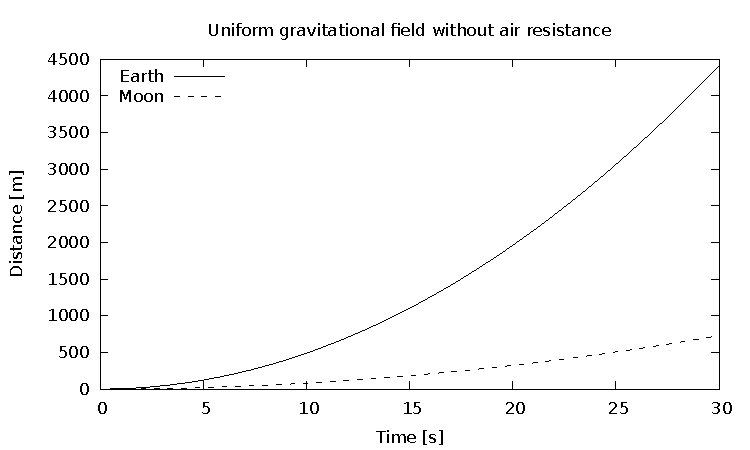
\includegraphics{gnuplot-bw}
% 	\caption{Černobílá varianta obrázku generovaného programem Gnuplot}\label{fig:gnuplot-bw}
% \end{figure}
% 
% \begin{figure}\centering
% 	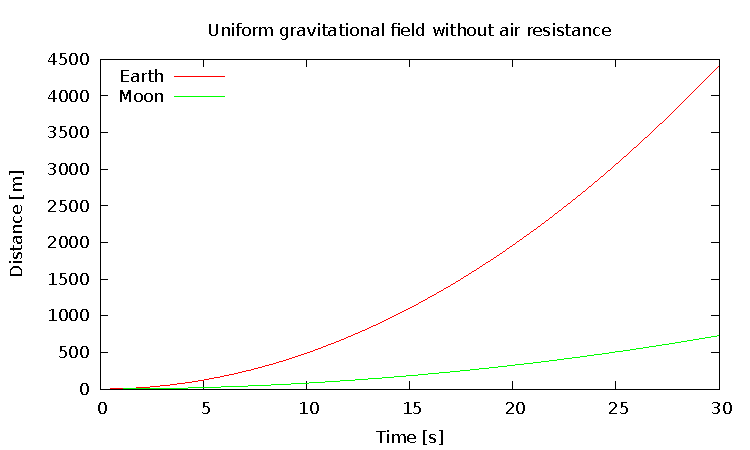
\includegraphics{gnuplot-col}
% 	\caption{Barevná varianta obrázku generovaného programem Gnuplot}\label{fig:gnuplot-col}
% \end{figure}
% 
% 
% \subsection{Tabulky}
% 
% Tabulky lze zadávat různě, např. v~prostředí \verb|tabular|, avšak pro jejich vkládání platí to samé, co pro obrázky -- použijte plovoucí prostředí, v~tomto případě \verb|table|. Například tabulka \ref{tab:matematika} byla vložena tímto způsobem.
% 
% \begin{table}\centering
% 	\caption[Příklad tabulky]{Zadávání matematiky}\label{tab:matematika}
% 	\begin{tabular}{|l|l|c|c|}\hline
% 		Typ		& Prostředí		& \LaTeX{}ovská zkratka	& \TeX{}ovská zkratka	\tabularnewline \hline \hline
% 		Text		& \verb|math|		& \verb|\(...\)|	& \verb|$...$|		\tabularnewline \hline
% 		Displayed	& \verb|displaymath|	& \verb|\[...\]|	& \verb|$$...$$|	\tabularnewline \hline
% 	\end{tabular}
% \end{table}
% 
% % % % % % % % % % % % % % % % % % % % % % % % % % % % 

% \chapter{Obsah přiloženého CD}

% %upravte podle skutecnosti

% \begin{figure}
% 	\dirtree{%
% 		.1 readme.txt\DTcomment{stručný popis obsahu CD}.
% 		.1 exe\DTcomment{adresář se spustitelnou formou implementace}.
% 		.1 src.
% 		.2 impl\DTcomment{zdrojové kódy implementace}.
% 		.2 thesis\DTcomment{zdrojová forma práce ve formátu \LaTeX{}}.
% 		.1 text\DTcomment{text práce}.
% 		.2 thesis.pdf\DTcomment{text práce ve formátu PDF}.
% 		.2 thesis.ps\DTcomment{text práce ve formátu PS}.
% 	}
% \end{figure}

\end{document}
